\chapter{Quantification of Spatial Self-Shielding Effects}
\label{chap:quantify}

%%%%%%%%%%%%%%%%%%%%%%%%%%%%%%%%%%%%%%%%%%%%%%%%%%%%%%%%%%%%%%%%%%%%%%%%%%%%%%%
\section{Pin-wise Spatial Homogenization Schemes}
\label{sec:chap8-pinwise-space-homogenize}

\subsection{Infinite Lattice Homogenization}

\subsection{Null Homogenization}

\subsection{Degenerate Homogenization}

\begin{figure}[h!]
\centering
\begin{subfigure}{.5\textwidth}
  \centering
  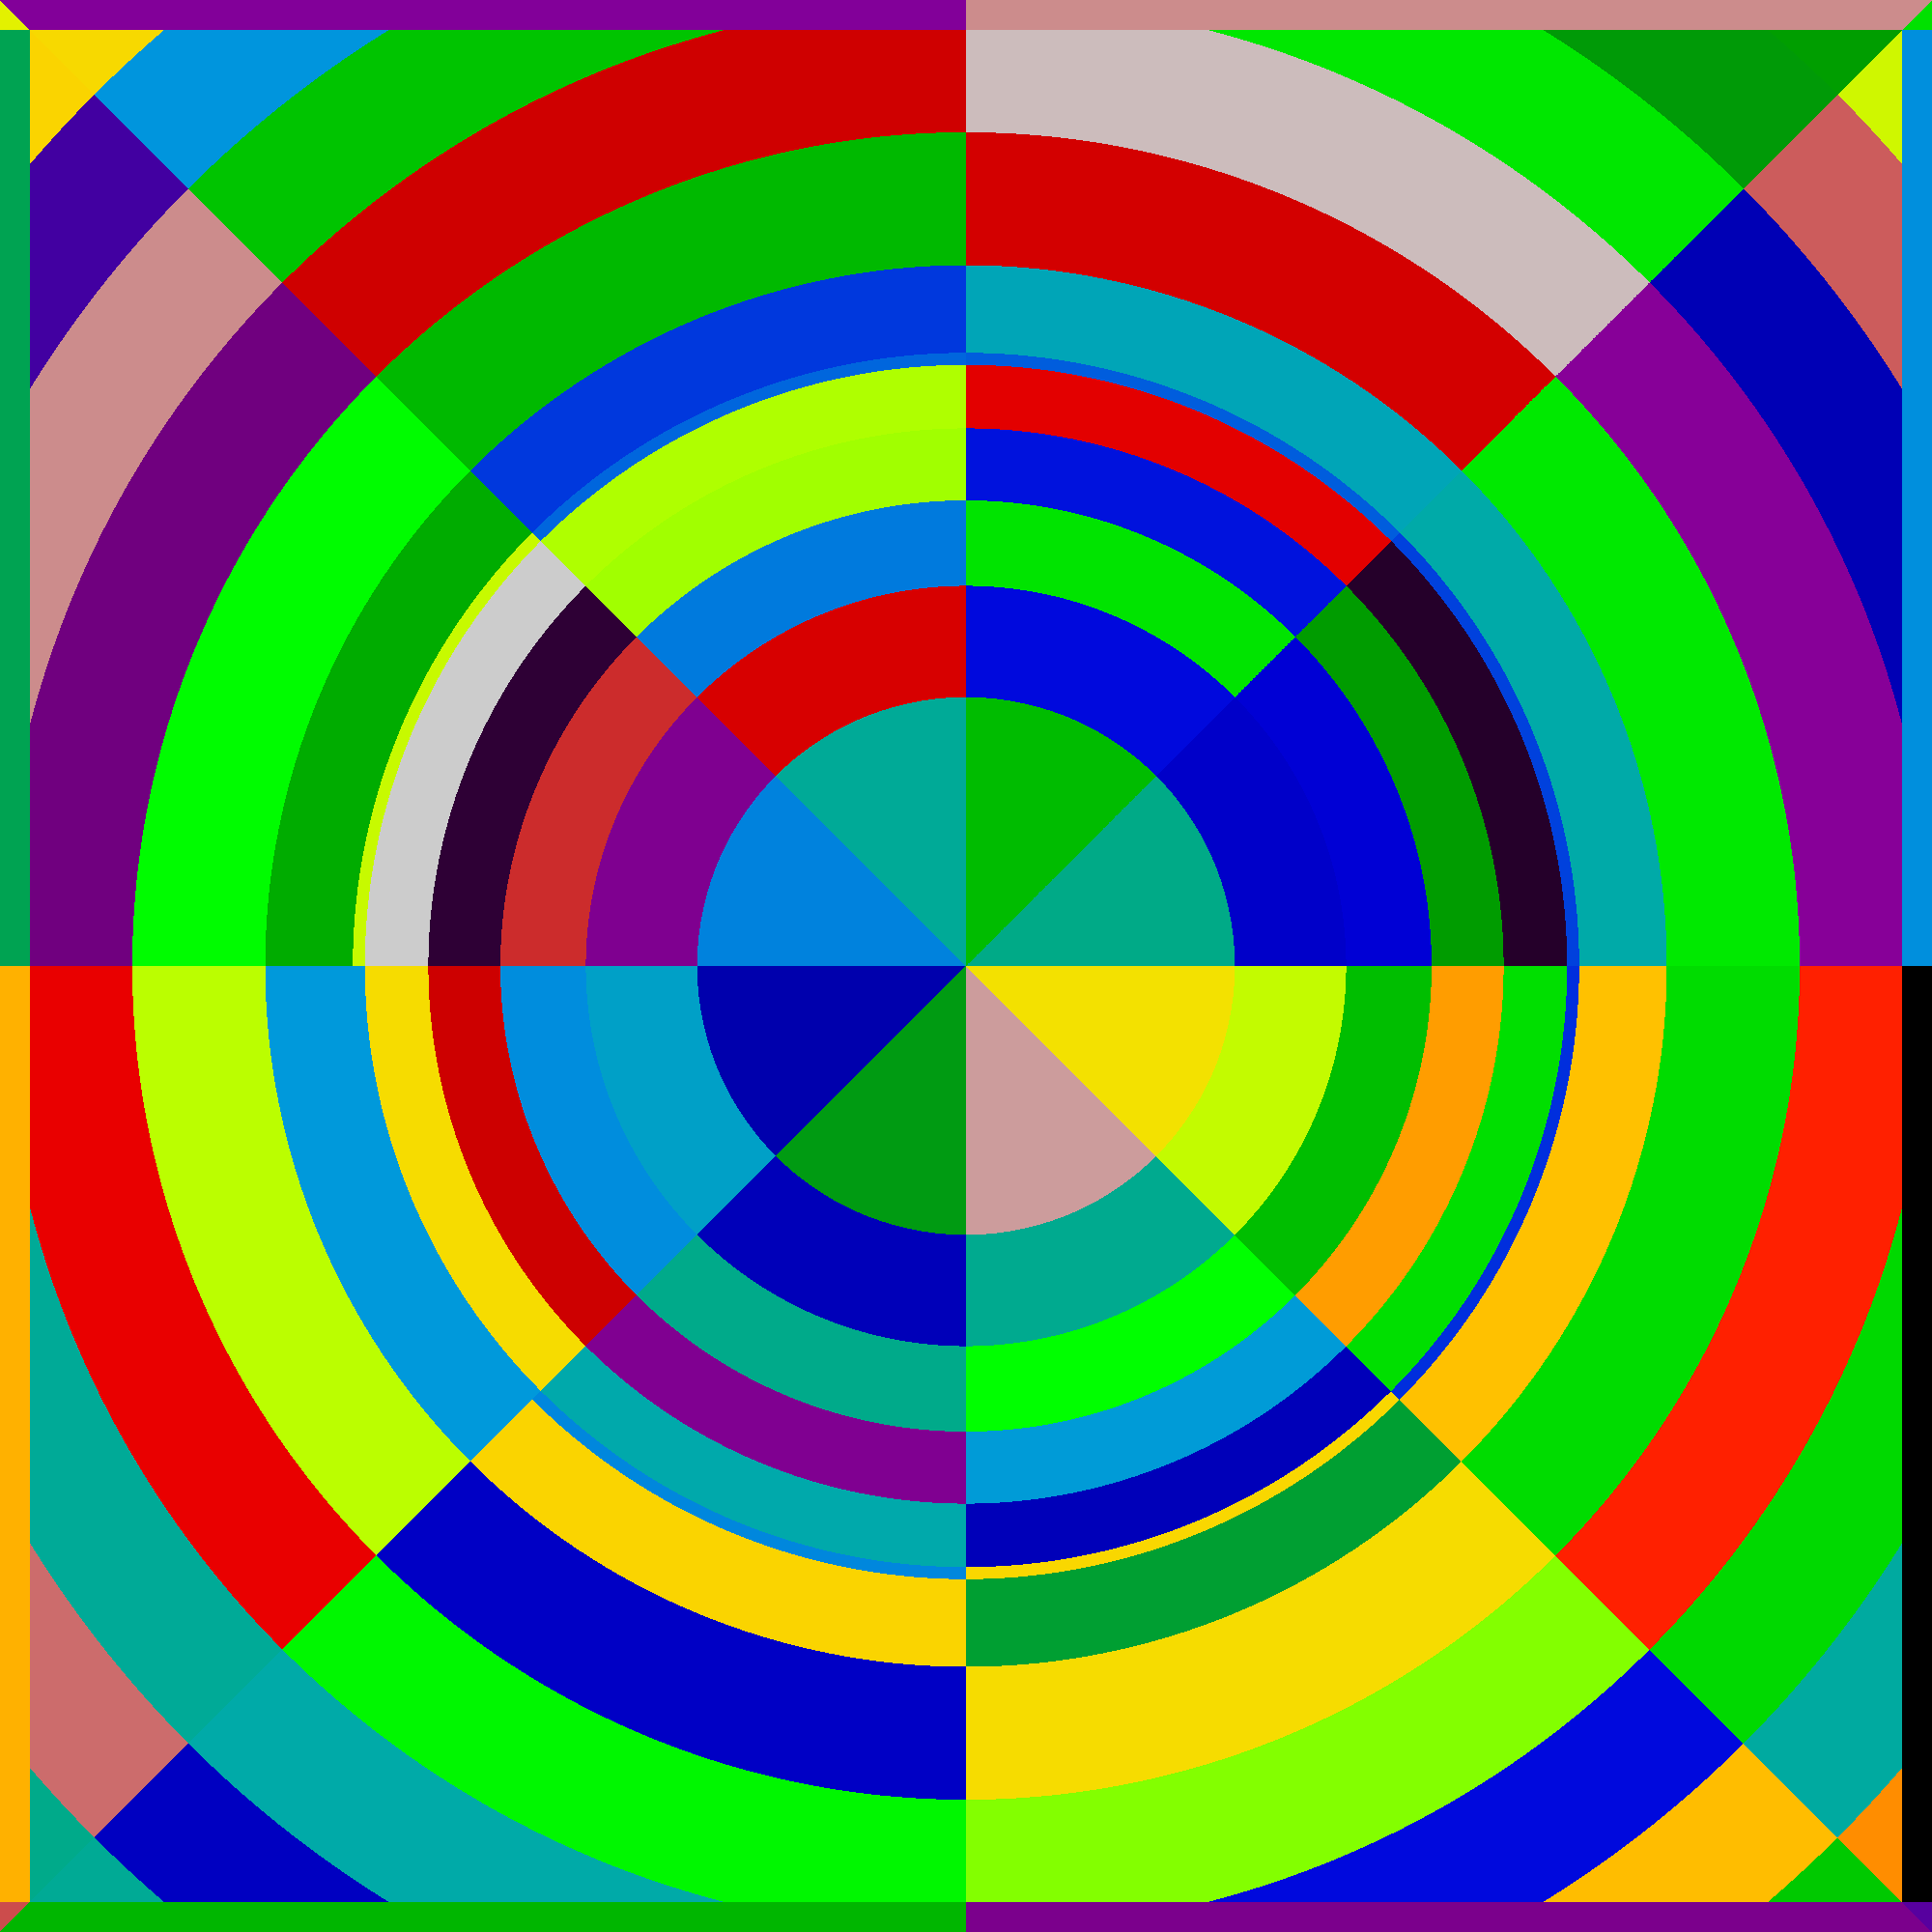
\includegraphics[width=0.9\linewidth]{figures/quantification/fsrs-fuel-pin}
  \caption{}
  \label{fig:chap8-pin-1.6}
\end{subfigure}%
\begin{subfigure}{.5\textwidth}
  \centering
  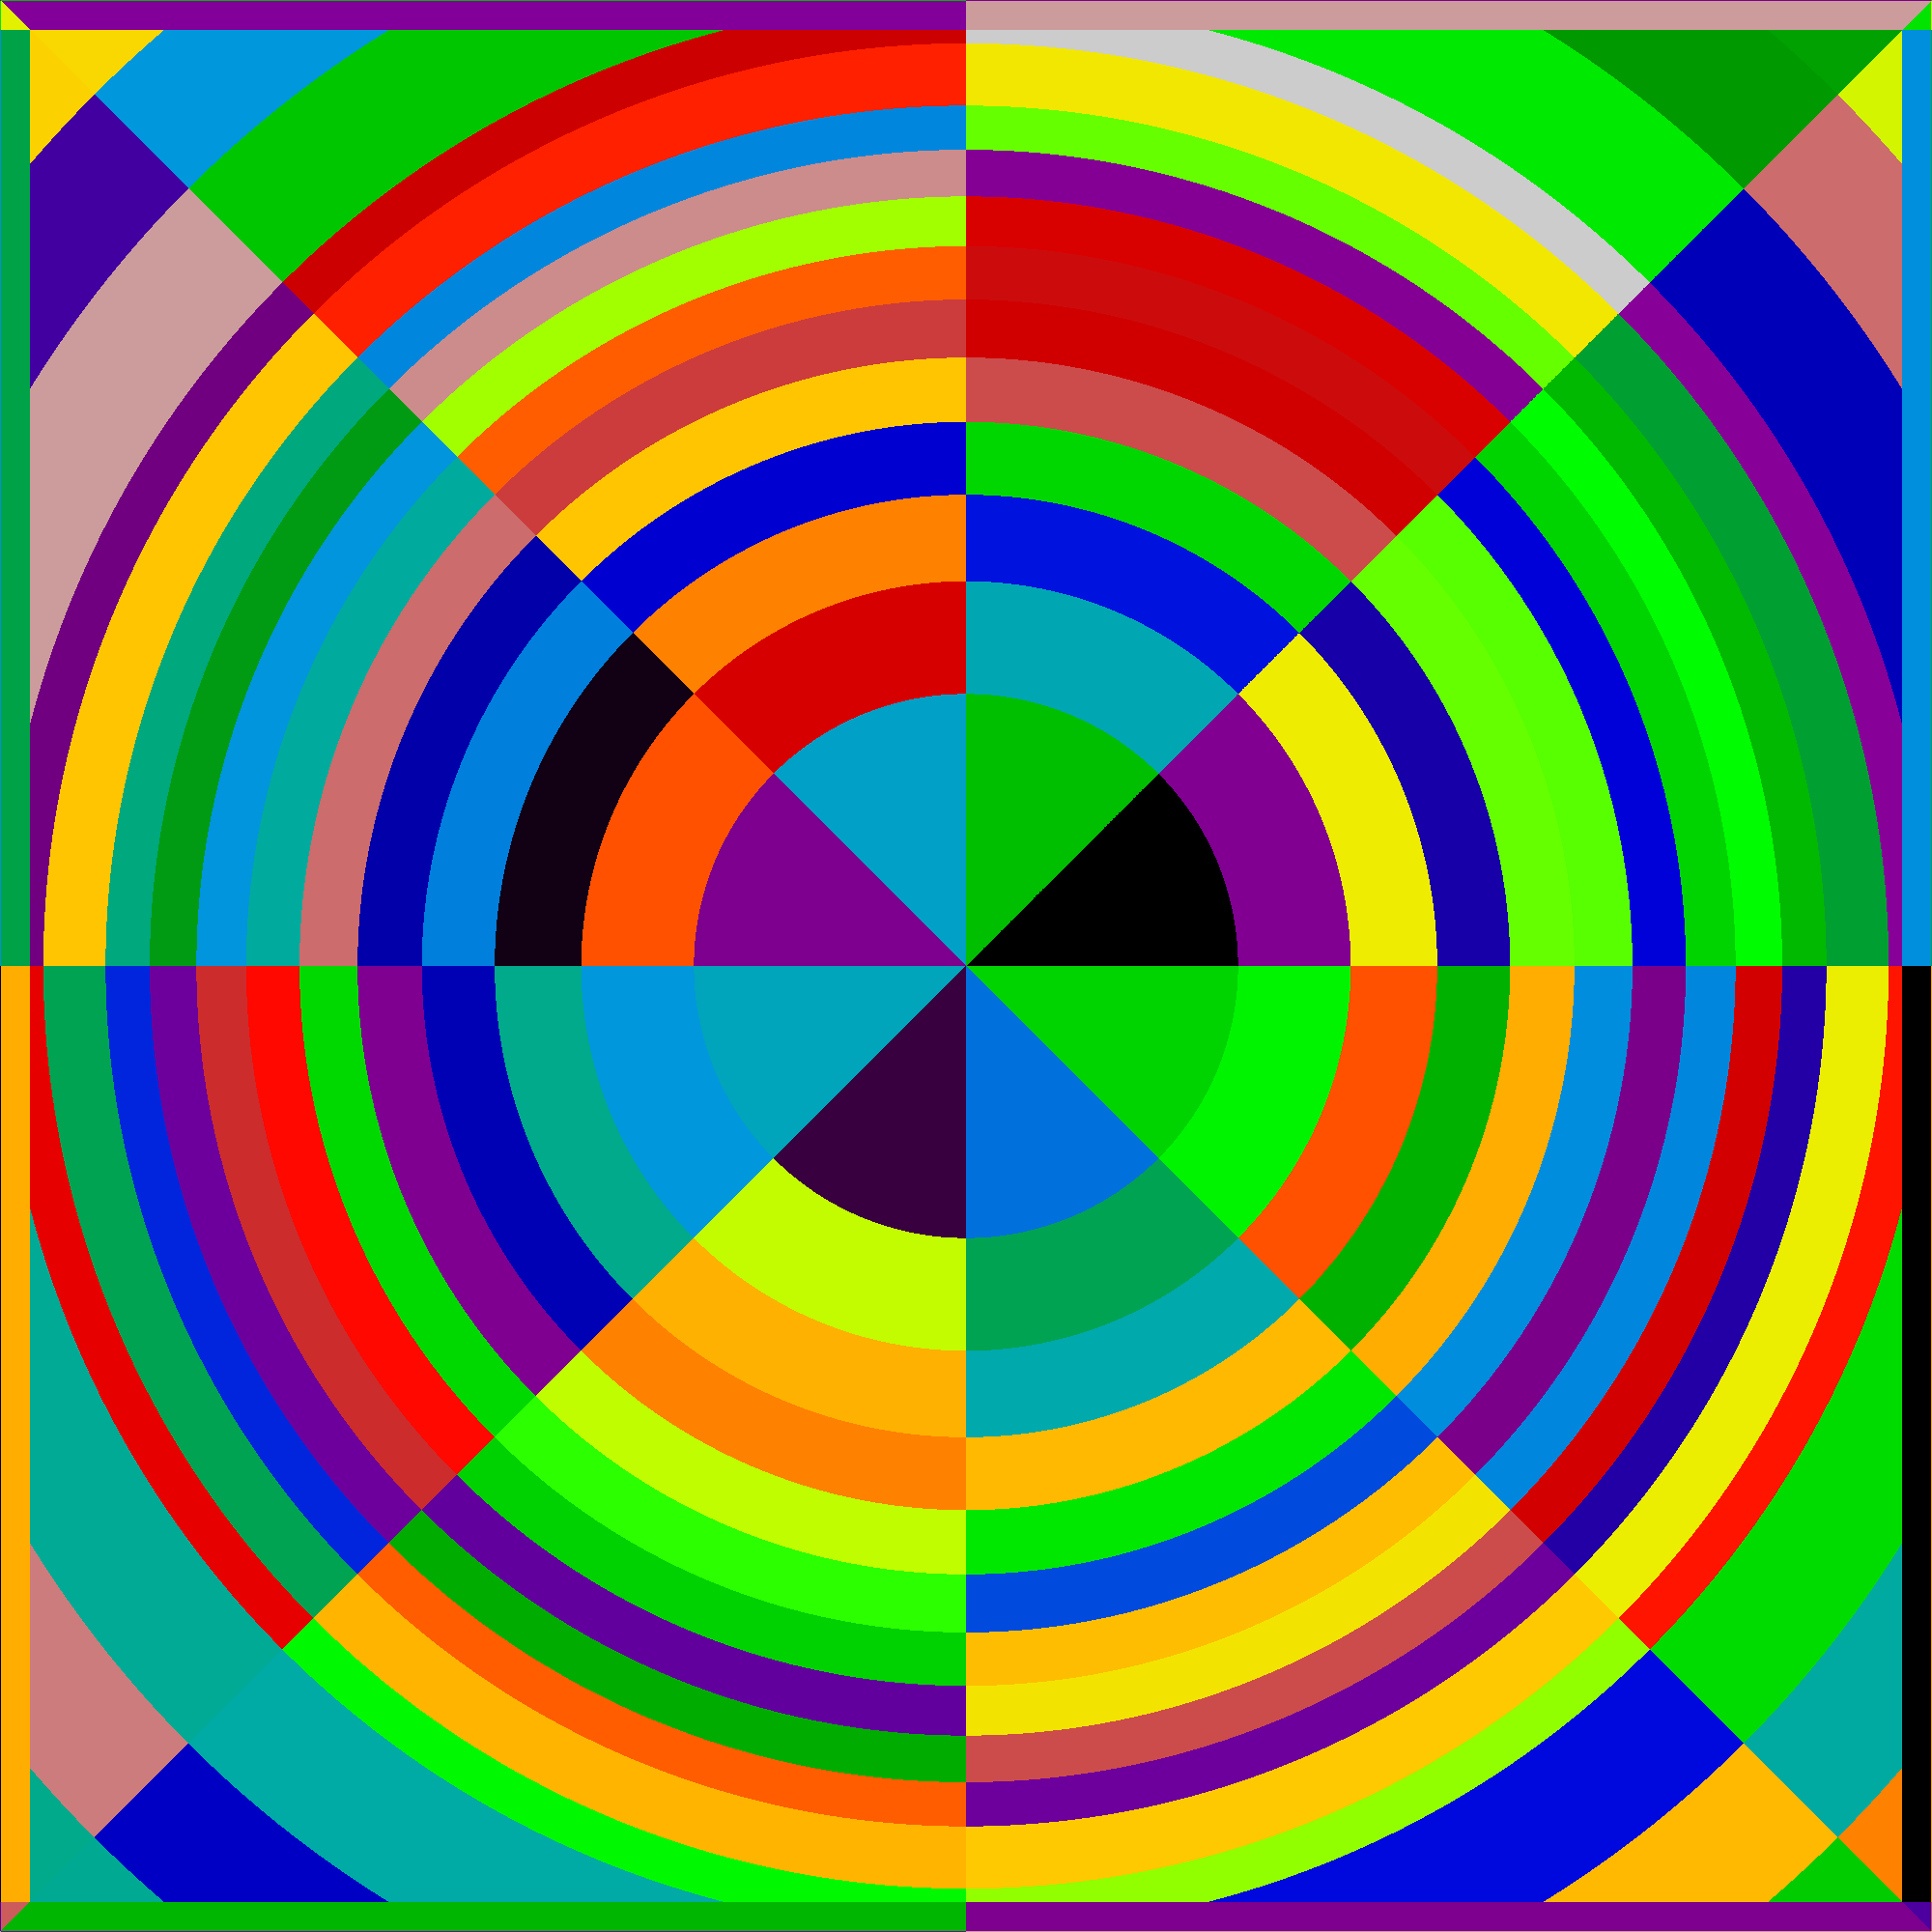
\includegraphics[width=0.9\linewidth]{figures/quantification/fsrs-crgt}
  \caption{}
  \label{fig:chap8-pin-crgt}
\end{subfigure}
\begin{subfigure}{.5\textwidth}
  \centering
  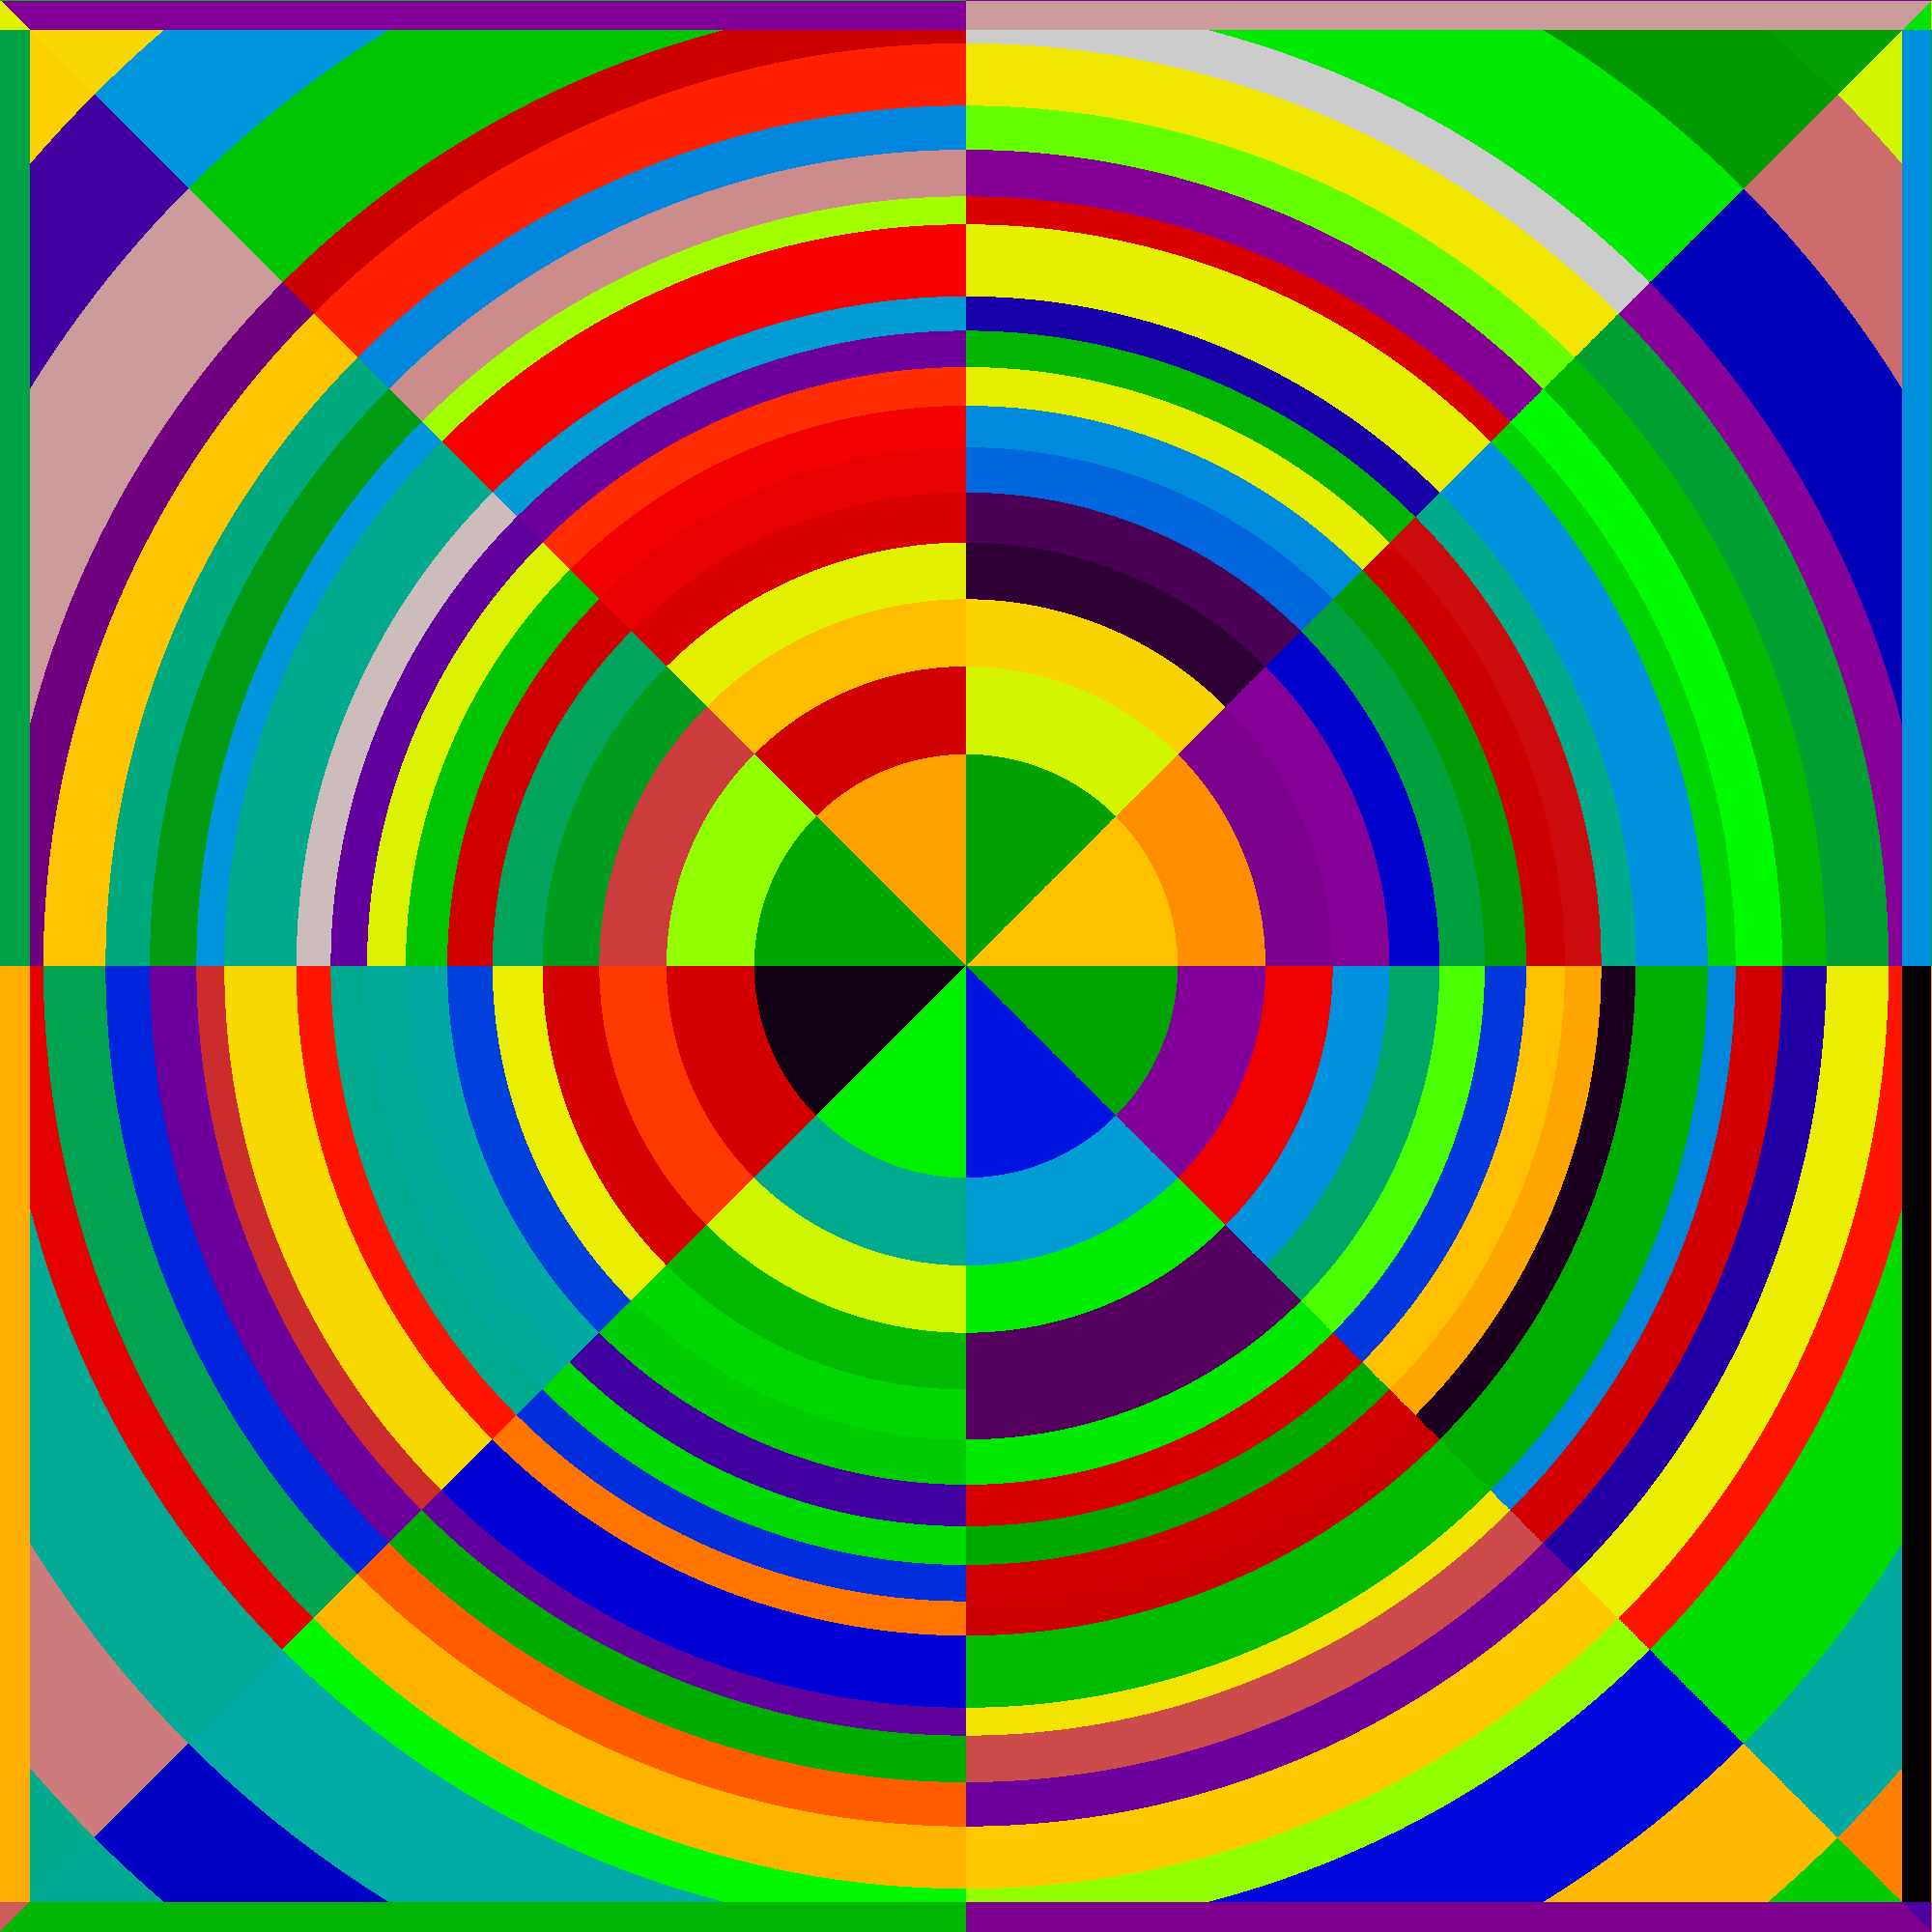
\includegraphics[width=0.9\linewidth]{figures/quantification/fsrs-instr-tube}
  \caption{}
  \label{fig:chap8-instr-tube}
\end{subfigure}%
\begin{subfigure}{.5\textwidth}
  \centering
  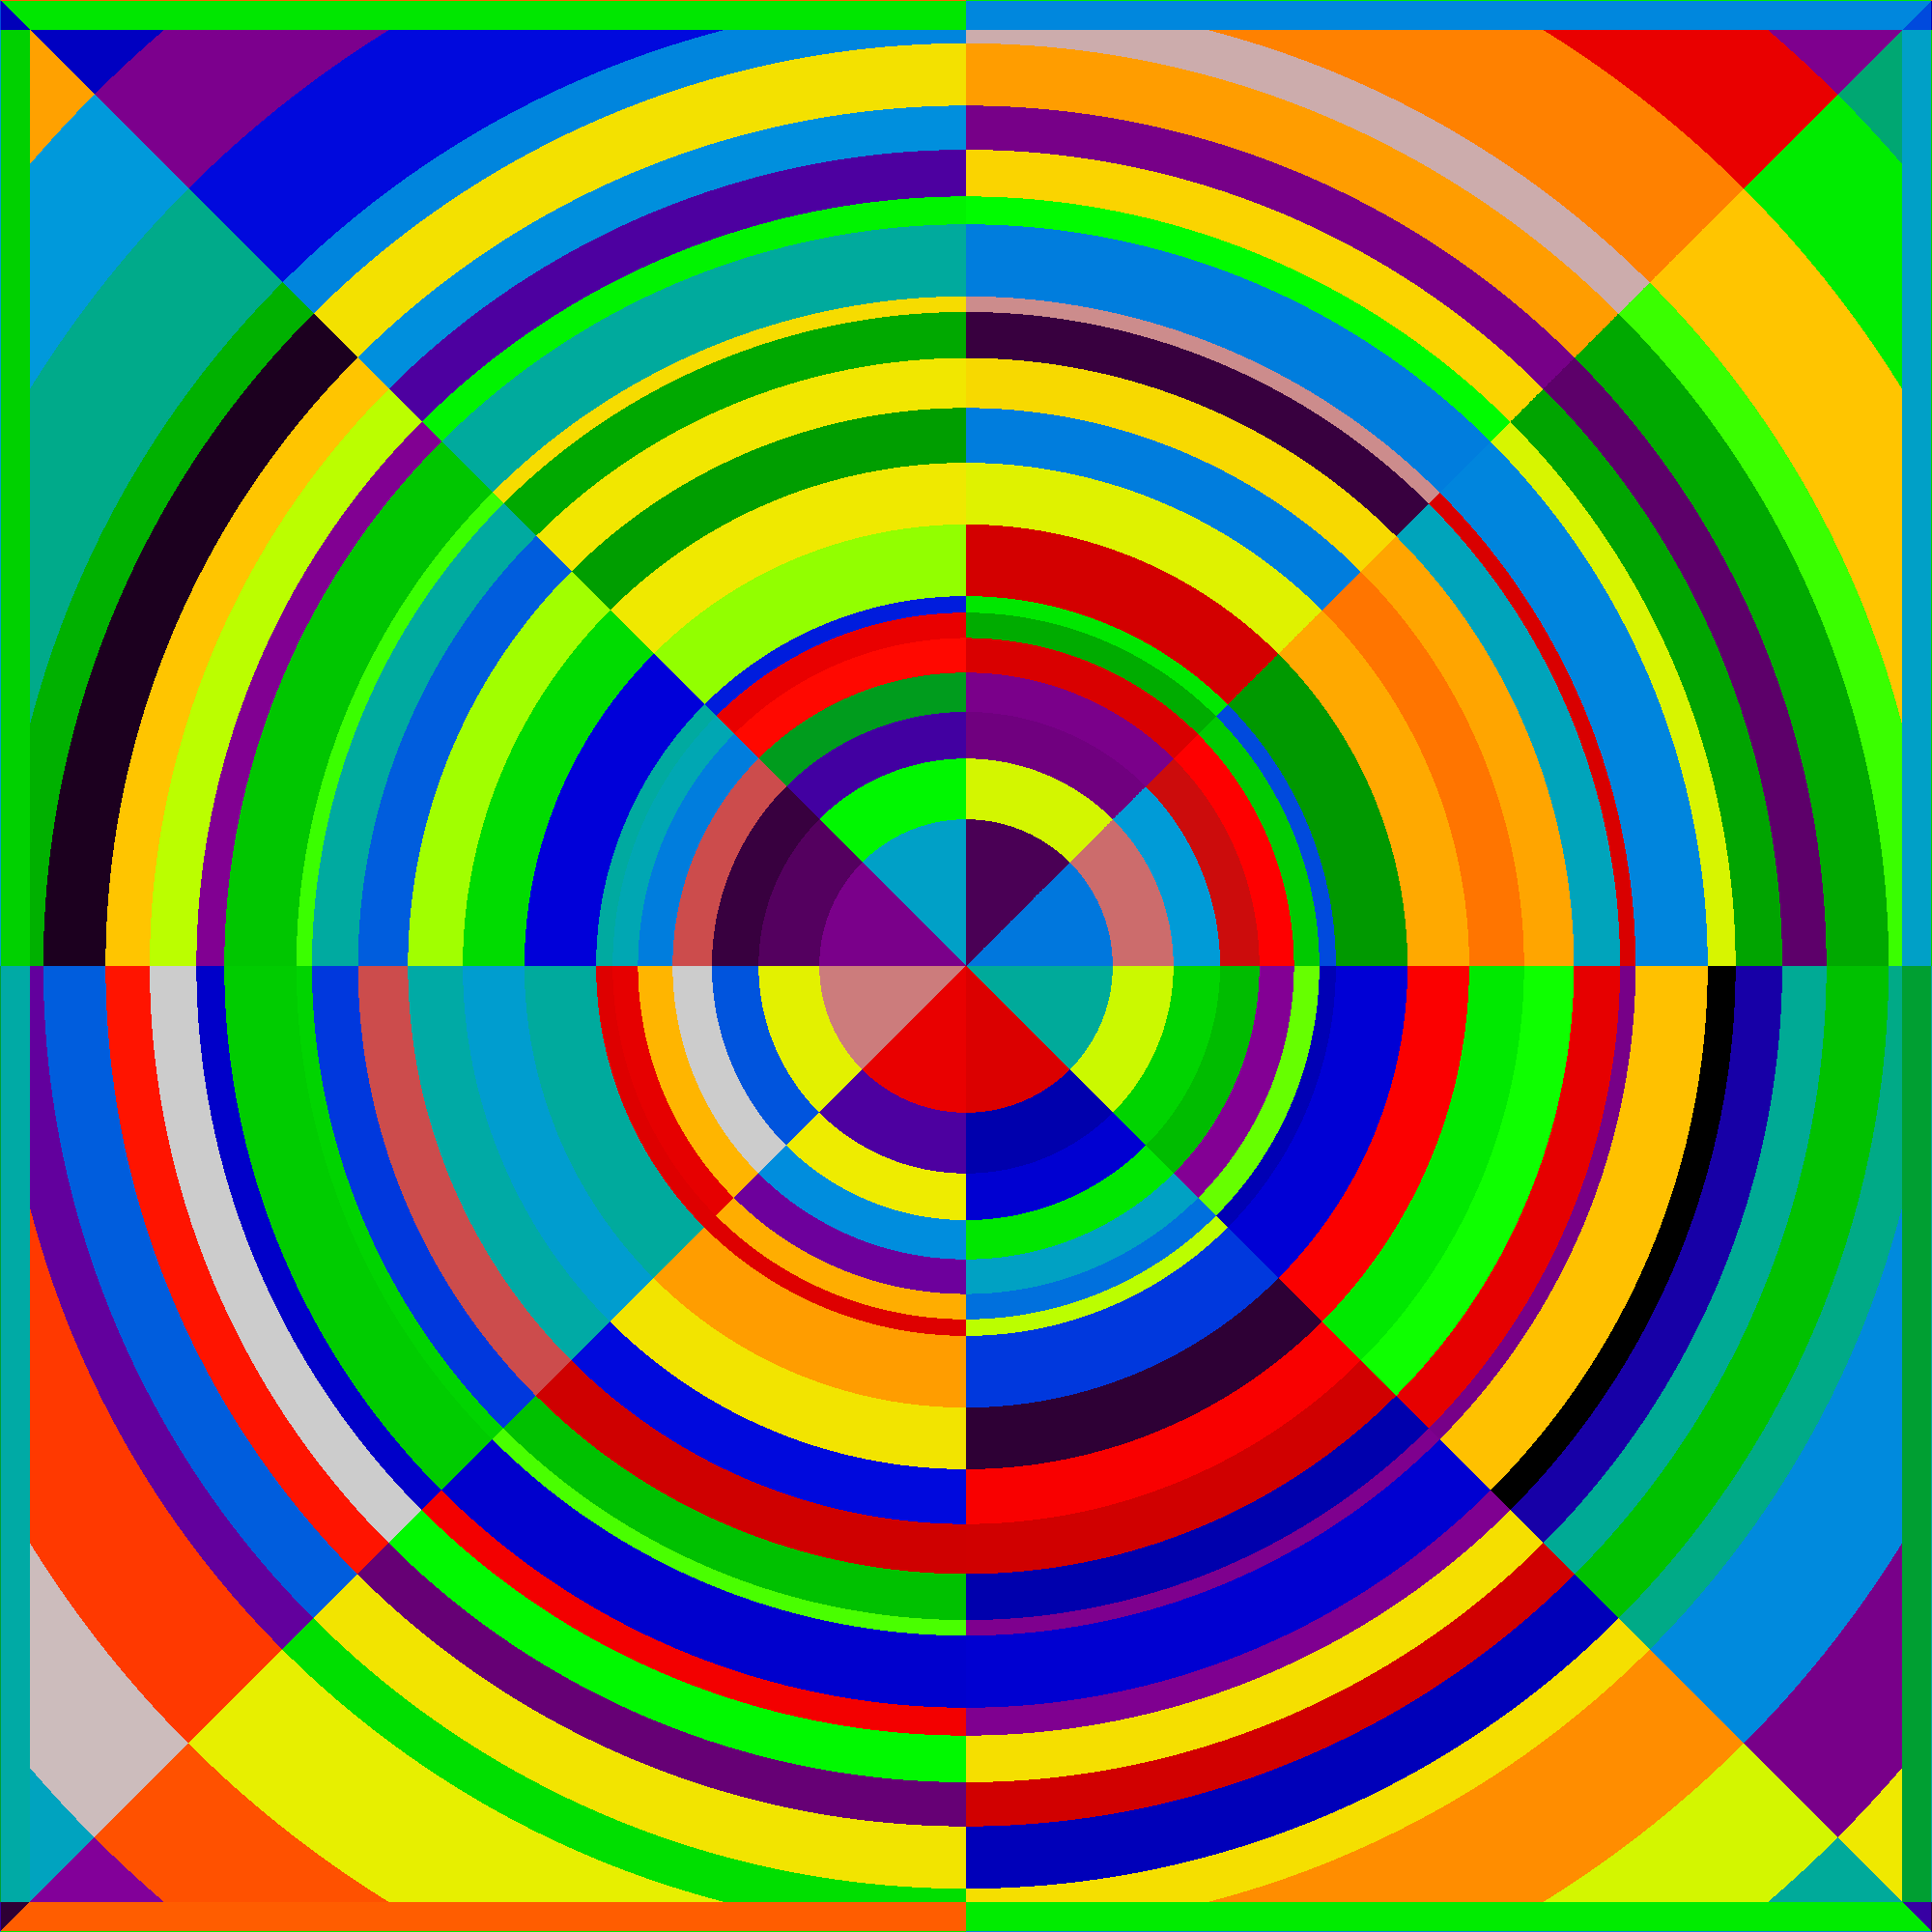
\includegraphics[width=0.9\linewidth]{figures/quantification/fsrs-bp}
  \caption{}
  \label{fig:chap8-bp}
\end{subfigure}%
\caption[BEAVRS pin cell FSR discretization]{1.6\% enriched fuel pin (a), control rod guide tube (b), instrument tube (c) and burnable poison (d).}
\label{fig:chap8-pin-cell-fsrs}
\end{figure}

\begin{figure}[h!]
\centering
\begin{subfigure}{0.5\textwidth}
  \centering
  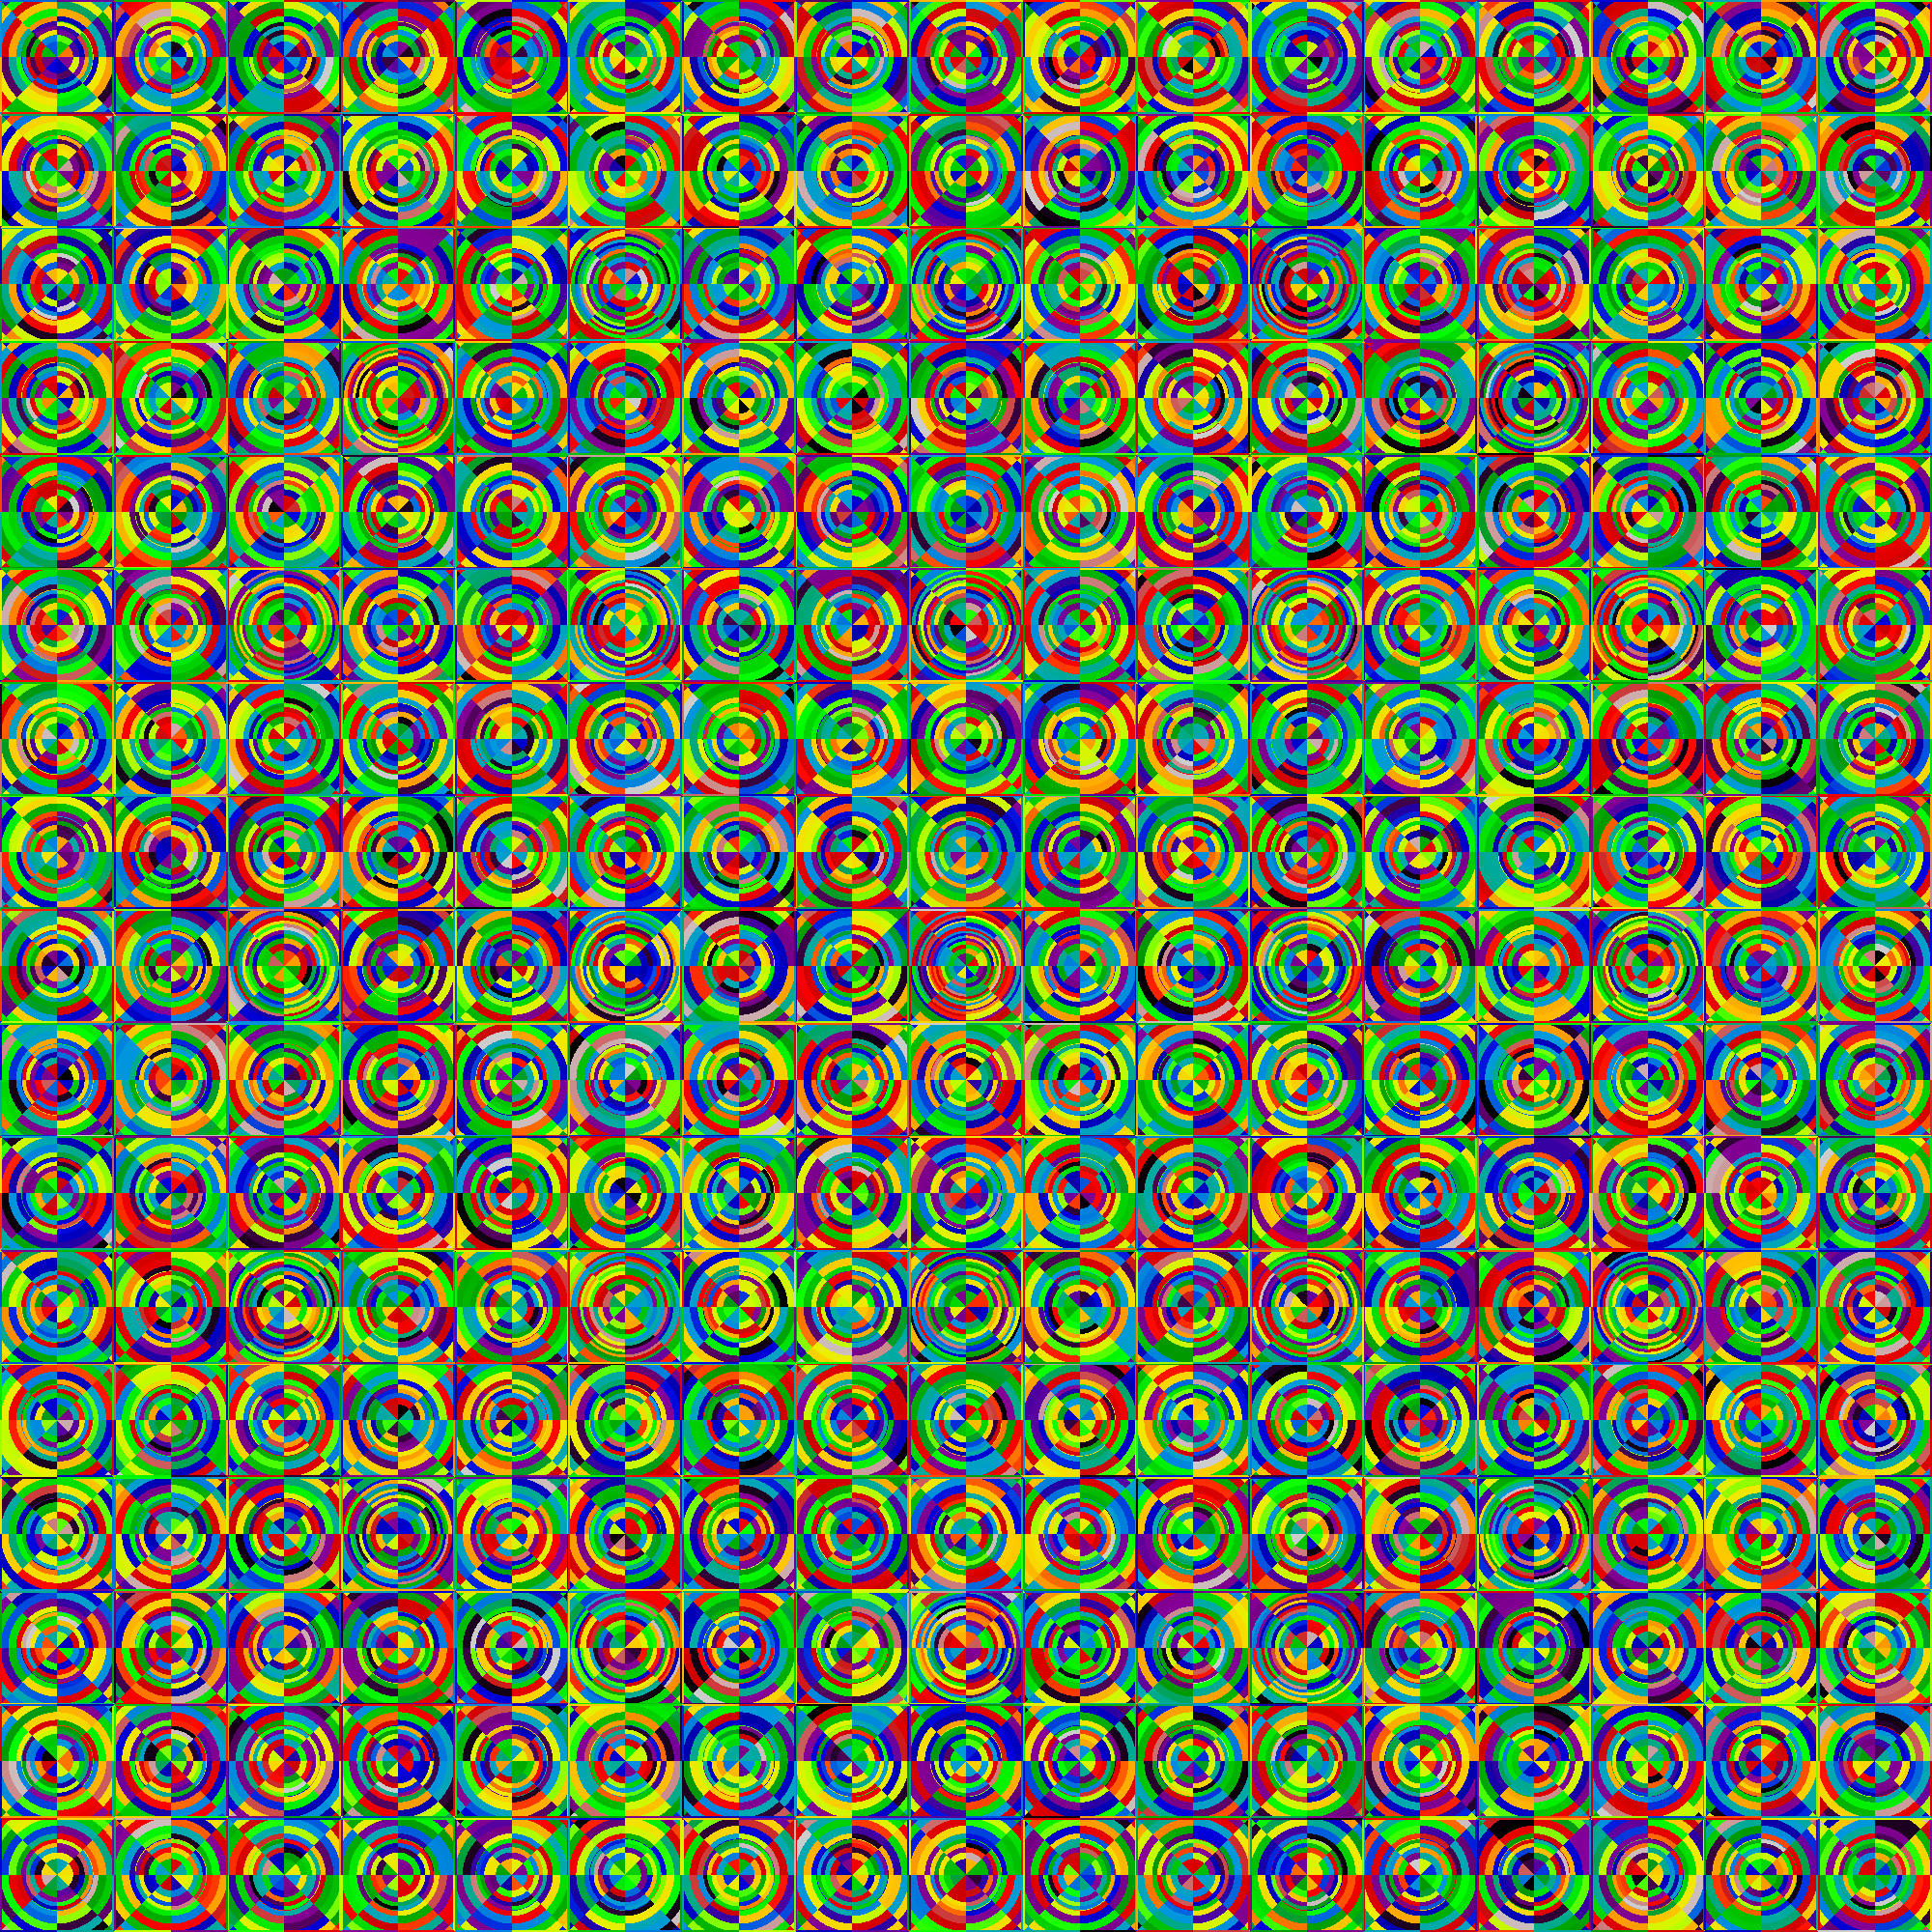
\includegraphics[width=0.9\linewidth]{figures/quantification/fsrs-assm-16}
  \caption{}
  \label{fig:chap8-assm-1.6}
\end{subfigure}%
\begin{subfigure}{0.5\textwidth}
  \centering
  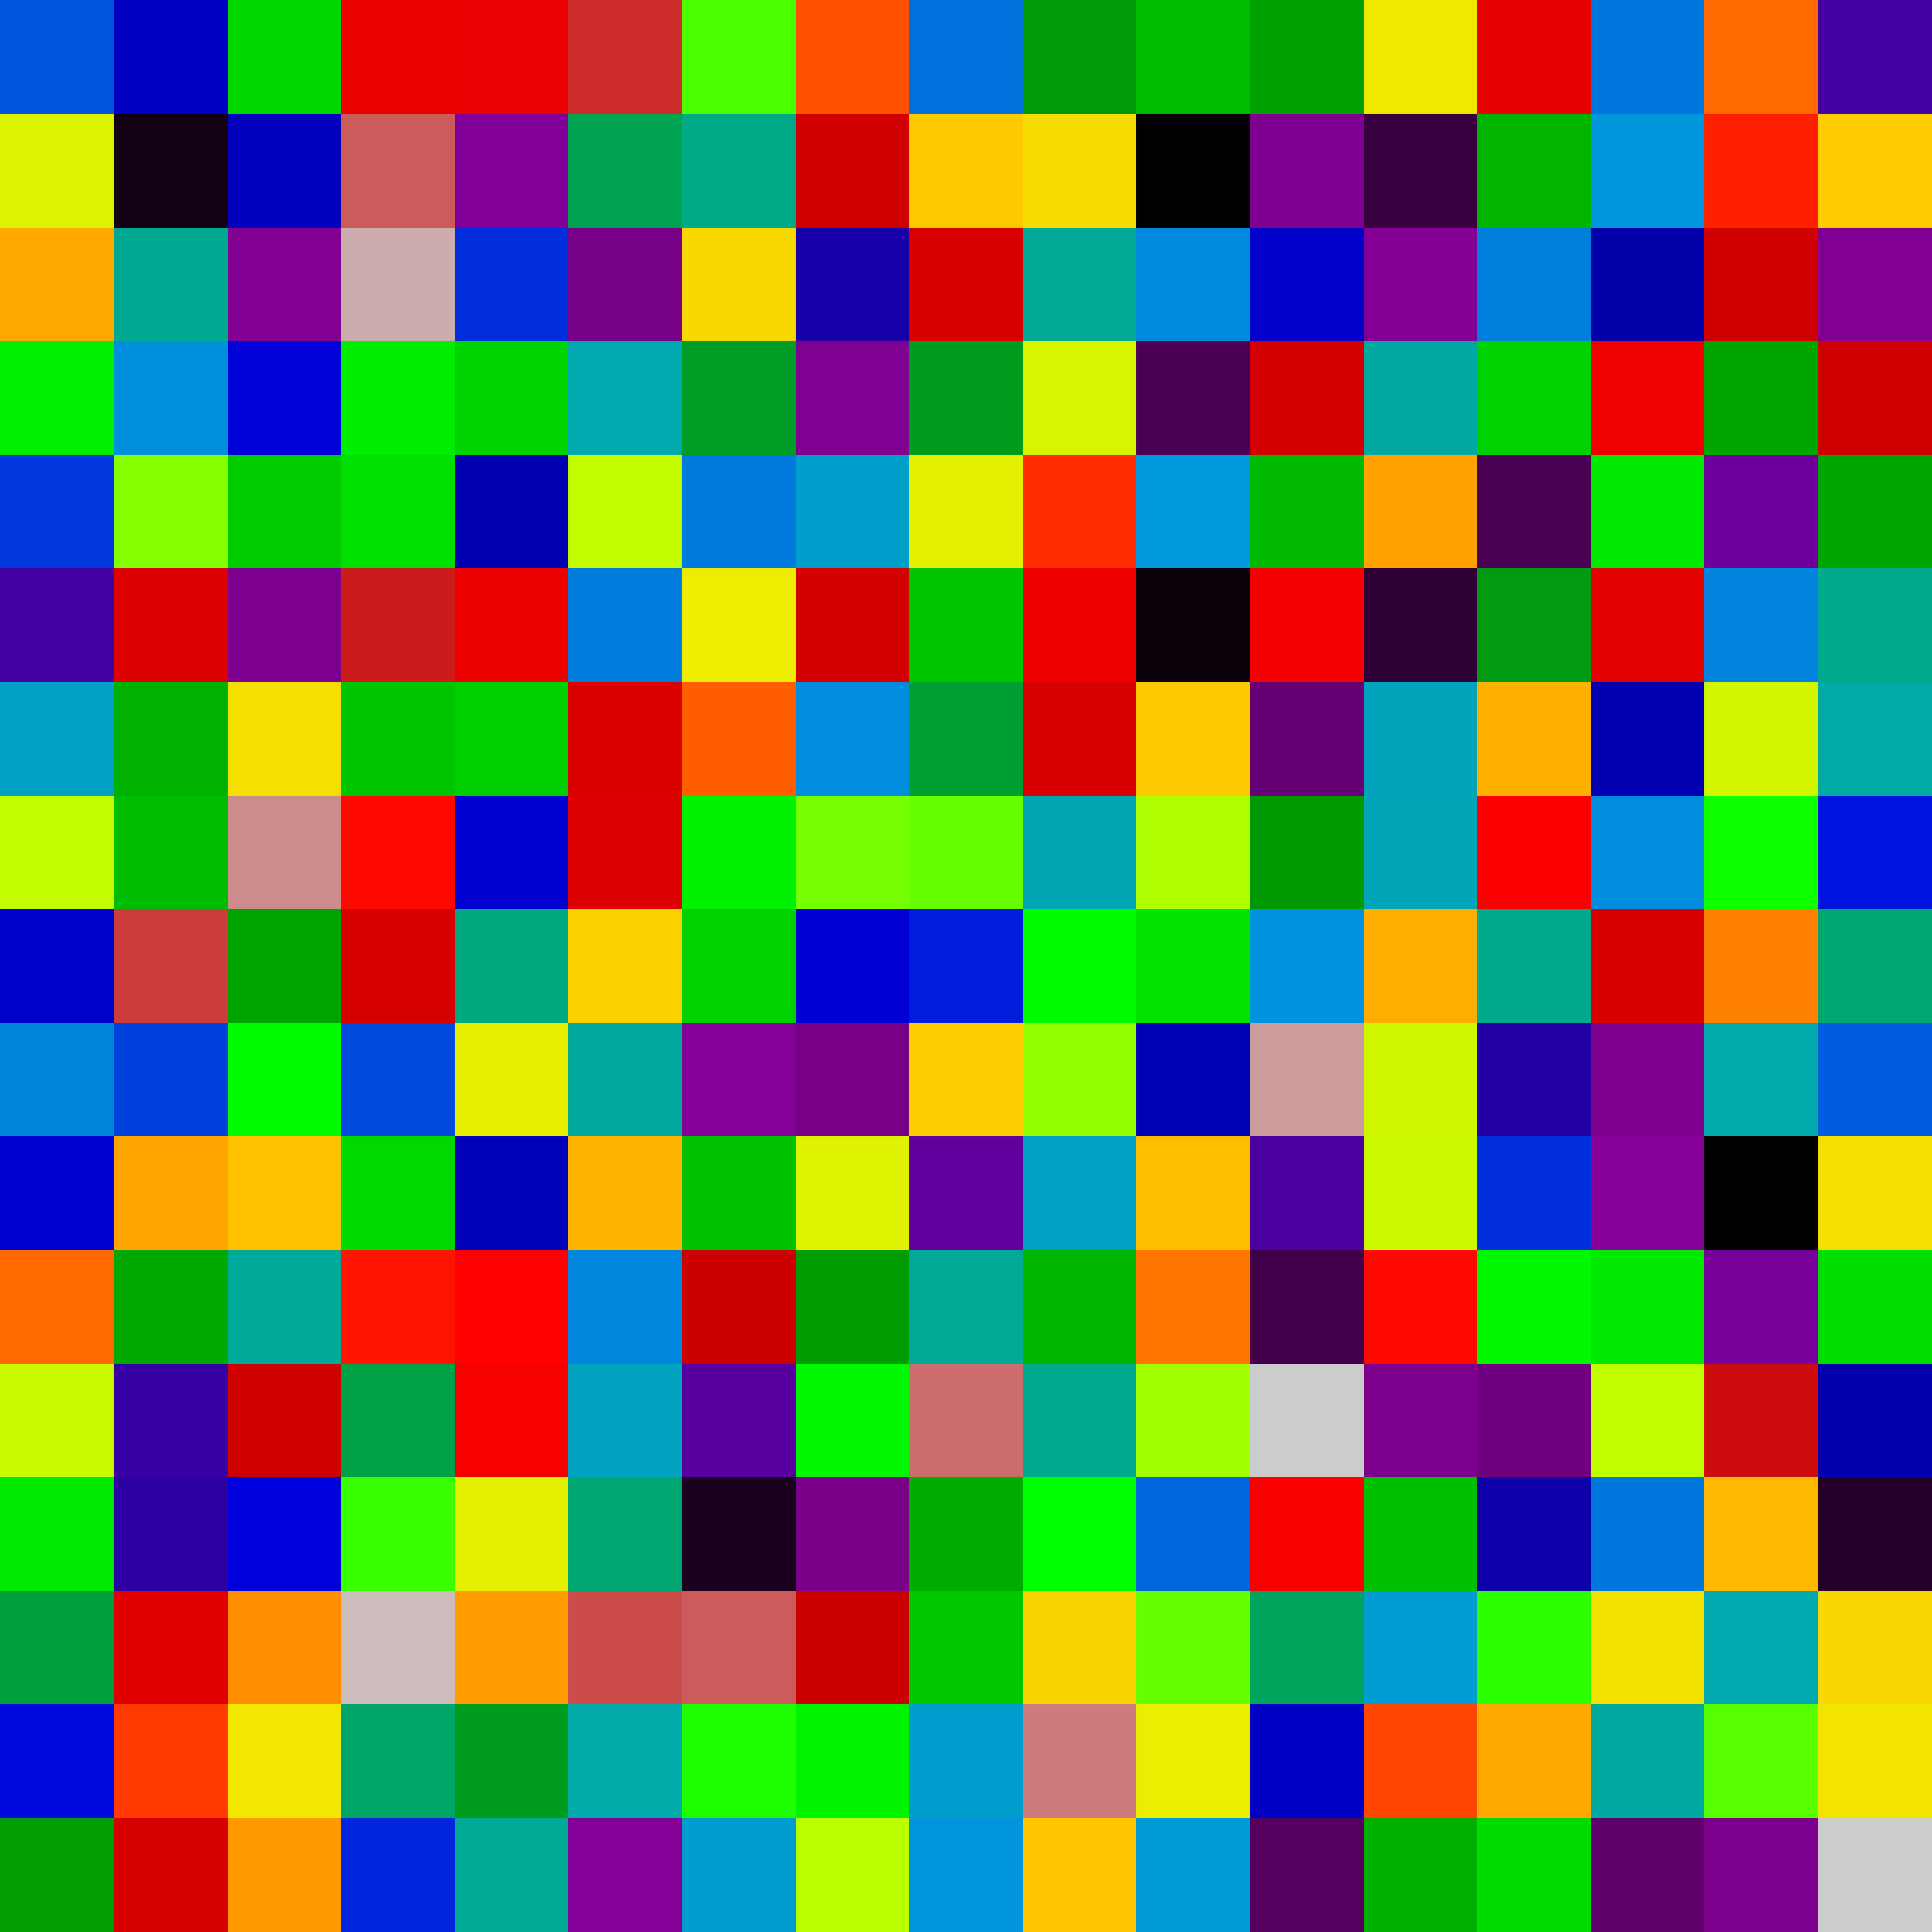
\includegraphics[width=0.9\linewidth]{figures/quantification/cmfd-cells-assm}
  \caption{}
  \label{fig:chap8-cmfd-cells}
\end{subfigure}
\caption[FSR discretization and CMFD cells for a fuel assembly]{\ac{FSR} discretization and \ac{CMFD} cells for a fuel assembly}
\label{fig:chap8-assm-fsrs-cmfd-cells}
\end{figure}

\begin{figure}[h!]
\centering
\begin{subfigure}{0.5\textwidth}
  \centering
  
\includegraphics[width=0.9\linewidth]{figures/quantification/fsrs-reflector}
  \caption{}
  \label{fig:chap8-assm-1.6}
\end{subfigure}%
\begin{subfigure}{0.5\textwidth}
  \centering
  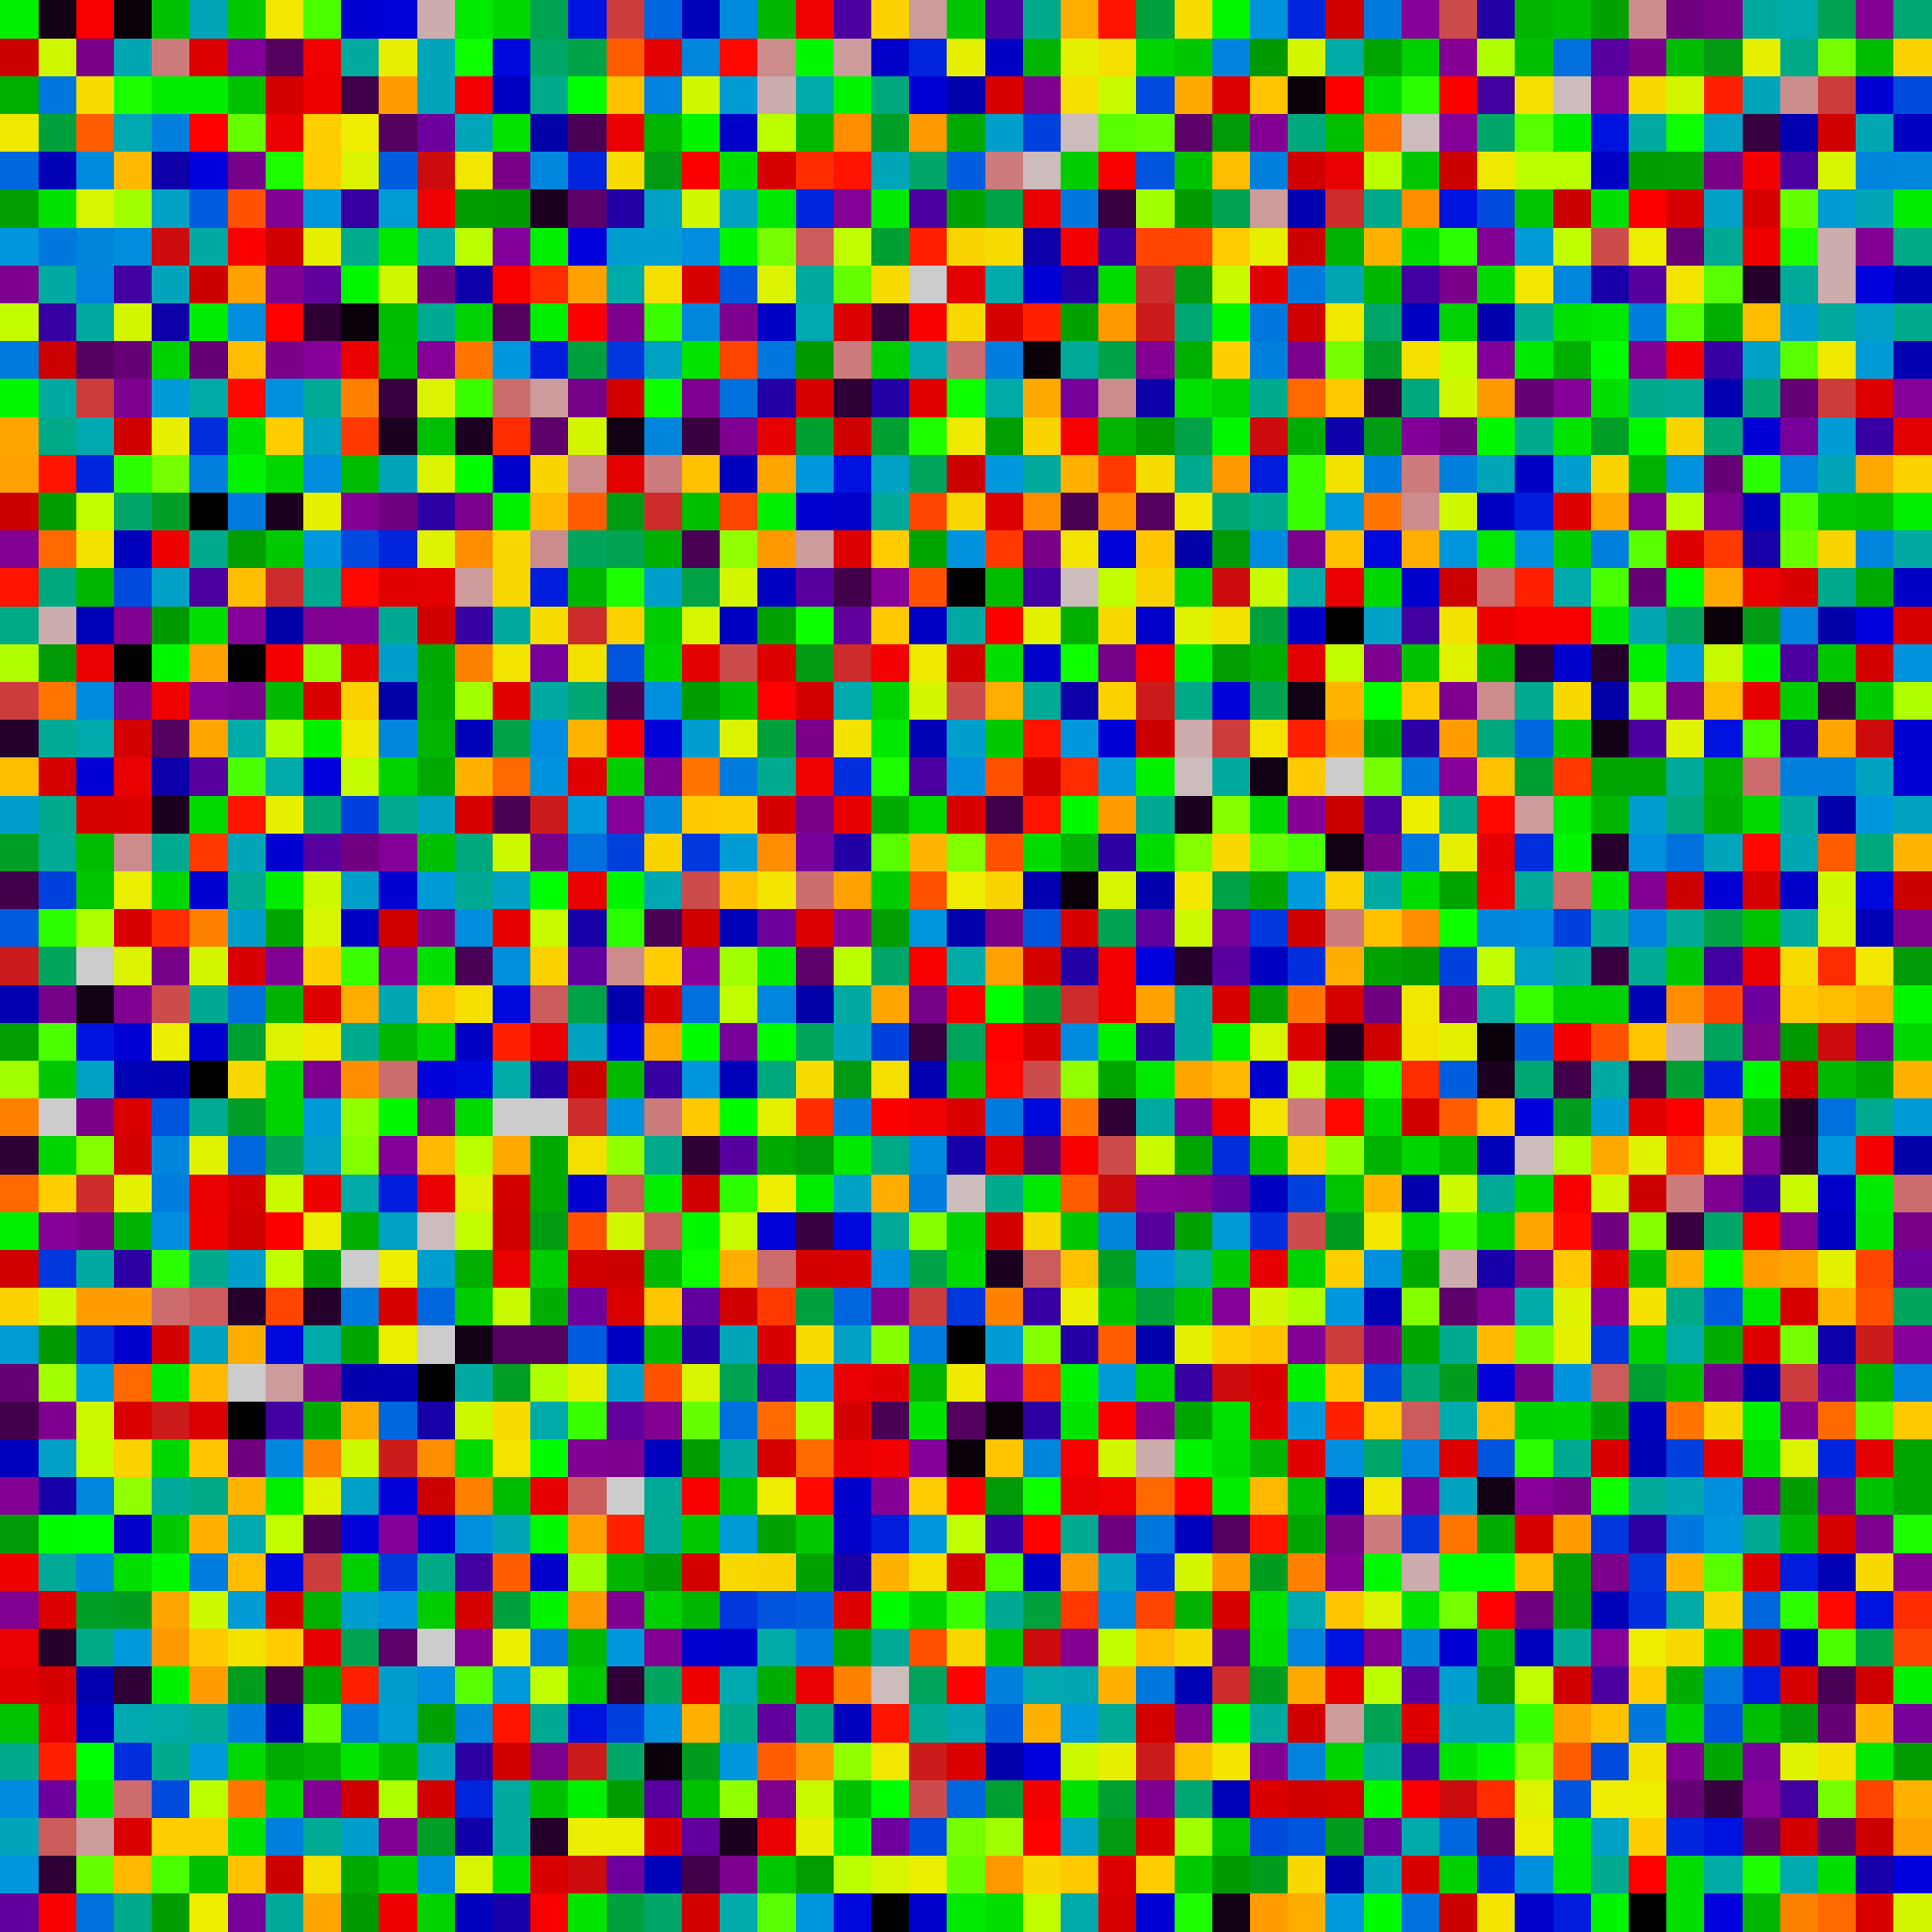
\includegraphics[width=0.9\linewidth]{figures/quantification/cmfd-cells-reflector}
  \caption{}
  \label{fig:chap8-cmfd-cells}
\end{subfigure}
\caption[FSR discretization and CMFD cells for a 2$\times$2 colorset with a reflector]{\ac{FSR} discretization and \ac{CMFD} cells for a 2$\times$2 colorset with a water reflector.}
\label{fig:chap8-assm-fsrs-cmfd-cells}
\end{figure}


%%%%%%%%%%%%%%%%%%%%%%%%%%%%%%%%%%%%%%%%%%%%%%%%%%%%%%%%%%%%%%%%%%%%%%%%%%%%%%%
\section{MGXS Convergence Rates}

\begin{itemize}[noitemsep]
  \item Plot evolution of rel. err. by batch for each homogenization scheme
  \begin{itemize}[noitemsep]
    \item groups with highest rel. err.
    \item reactions with greatest contribution to eigenvalue (U-238 capture)
    \item total (track-length) vs. scattering matrices (analog)    
    \item which group structure(s)?
 \end{itemize}
  \item compare to pin power convergence rates in preceding chapter
\end{itemize}


%%%%%%%%%%%%%%%%%%%%%%%%%%%%%%%%%%%%%%%%%
\section{Analysis of Multi-Group Results}
\label{sec:chap8-mg-results}


%%%%%%%%%%%%%%%%%%%%%%%%
\subsection{Eigenvalues}
\label{subsec:chap8-eigenvalues}

\begin{table}[h!]
  \centering
  \caption[OpenMOC eigenvalue bias for heterogeneous benchmarks]{OpenMOC eigenvalue bias $\Delta\rho$ for heterogeneous benchmarks with infinite, null and degenerate spatial homogenization schemes.}
  \small
  \label{table:chap8-openmoc-eigenvalues}
  \vspace{6pt}
  \begin{tabular}{l l S[table-format=6.1]}
  \toprule
  {\cellcolor{lightgray} \bf Benchmark} &
  {\cellcolor{lightgray} \bf \ac{MGXS} Scheme} &
  \multicolumn{1}{S[table-format=6.1]}{\cellcolor{lightgray}{$\bm{\Delta\rho}$}} \\
  \midrule
  \multirow{3}{*}{1.6\% Enr. Assembly (no \ac{BP}s)} & Infinite & 987 \\
  & Null & \\
  & Degenerate & \\
  \midrule
  \multirow{3}{*}{3.1\% Enr. Assembly (no \ac{BP}s)} & Infinite & 344 \\
  & Null & \\
  & Degenerate & \\
  \midrule
  \multirow{3}{*}{3.1\% Enr. Assembly (20 \ac{BP}s)} & Infinite & 530 \\
  & Null & \\
  & Degenerate & \\
  \midrule
  \multirow{3}{*}{2$\times$2 Colorset} & Infinite & 196 \\
  & Null & \\
  & Degenerate & \\
  \midrule
  \multirow{3}{*}{2$\times$2 Colorset w/ Reflector} & Infinite & 462\\
  & Null & \\
  & Degenerate & \\
  \midrule
  \multirow{3}{*}{\ac{BEAVRS} Full Core} & Infinite & 497 \\
  & Null & \\
  & Degenerate & \\
  \bottomrule
\end{tabular}
\end{table}

\begin{itemize}[noitemsep]
  \item table of eigenvalue bias with converged MGXS for each benchmark
  \begin{itemize}[noitemsep]
    \item infinite vs. null vs. degenerate
    \item by energy group structure?
  \end{itemize}
  \item plots of keff convergence by batch for each benchmark
  \begin{itemize}[noitemsep]
    \item infinite vs. null vs. degenerate (null and degenerate are identical)
    \item by energy group structure?
  \end{itemize}
\end{itemize}

%%%%%%%%%%%%%%%%%%%%%%%%%%
\subsection{Fission Rates}
\label{subsec:chap8-fiss-rates}

\begin{table}[h!]
  \centering
  \caption[OpenMOC fission rate errors for heterogeneous benchmarks]{OpenMOC fission rate errors for heterogeneous benchmarks with infinite, null and degenerate spatial homogenization schemes.}
  \small
  \label{table:chap8-openmoc-fiss-rates}
  \vspace{6pt}
  \begin{tabular}{l l S[table-format=4.1] S[table-format=4.1]}
  \toprule
  {\cellcolor{lightgray} \bf Benchmark} &
  {\cellcolor{lightgray} \bf \ac{MGXS} Scheme} &
  \multicolumn{1}{S[table-format=6.1]}{\cellcolor{lightgray} \textbf{Max Error [\%]}} &
  \multicolumn{1}{S[table-format=6.1]}{\cellcolor{lightgray} \textbf{Mean Error [\%]}} \\
  \midrule
  \multirow{3}{*}{1.6\% Enr. Assembly (no \ac{BP}s)} & Infinite & 987 & 987 \\
  & Null & & \\
  & Degenerate & & \\
  \midrule
  \multirow{3}{*}{3.1\% Enr. Assembly (no \ac{BP}s)} & Infinite & 344 & 344 \\
  & Null & & \\
  & Degenerate & & \\
  \midrule
  \multirow{3}{*}{3.1\% Enr. Assembly (20 \ac{BP}s)} & Infinite & 530 & 580 \\
  & Null & & \\
  & Degenerate & & \\
  \midrule
  \multirow{3}{*}{2$\times$2 Colorset} & Infinite & 196 & 196 \\
  & Null & & \\
  & Degenerate & & \\
  \midrule
  \multirow{3}{*}{2$\times$2 Colorset w/ Reflector} & Infinite & 462 & 462 \\
  & Null & & \\
  & Degenerate & & \\
  \midrule
  \multirow{3}{*}{\ac{BEAVRS} Full Core} & Infinite & 497 & 497 \\
  & Null & & \\
  & Degenerate & & \\
  \bottomrule
\end{tabular}
\end{table}

\begin{itemize}[noitemsep]
  \item convergence rates for max/mean rel. err. for each benchmark
  \begin{itemize}[noitemsep]
    \item infinite vs. null vs. degenerate
    \item by energy group structure?
  \end{itemize}
  \item 2D heat maps of error distributions for each benchmark
  \begin{itemize}[noitemsep]
    \item infinite vs. null vs. degenerate
    \item by energy group structure?
  \end{itemize}
  \item bar charts of max/mean errors for each benchmark
  \begin{itemize}[noitemsep]
    \item infinite vs. null vs. degenerate
    \item by energy group structure?
  \end{itemize}
  \item histograms of error distributions for each benchmark
  \begin{itemize}[noitemsep]
    \item infinite vs. null vs. degenerate
    \item by energy group structure?
  \end{itemize}
\end{itemize}

%%%%%%%%%%%%%%%%%%%%%%%%%%%%%%%%%%%%%%%%%%%%%
\subsection{U-238 Capture Rate Distributions}
\label{subsec:chap8-capt-rates}

\begin{table}[h!]
  \centering
  \caption[OpenMOC U-238 capture rate errors for heterogeneous benchmarks]{OpenMOC U-238 capture rate errors for heterogeneous benchmarks with infinite, null and degenerate spatial homogenization schemes.}
  \small
  \label{table:chap8-openmoc-capt-rates}
  \vspace{6pt}
  \begin{tabular}{l l S[table-format=6.1] S[table-format=6.1] S[table-format=6.1]}
  \toprule
  \multirow{-2}{*}{\cellcolor{lightgray} \bf Benchmark} &
  \multirow{-2}{*}{\cellcolor{lightgray} \bf \ac{MGXS} Scheme} &
  \multicolumn{3}{S[table-format=6.1]}{\cellcolor{lightgray} \textbf{Max Error [\%]}} \\
  & & {\cellcolor{lightgray} \bf 2-Group} &
  {\cellcolor{lightgray} \bf 8-Group} &
  {\cellcolor{lightgray} \bf 70-Group} \\
%  \multicolumn{1}{S[table-format=6.1]}{\cellcolor{lightgray} \textbf{Mean Error [\%]}} \\
  \midrule
  \multirow{3}{*}{\parbox{2.5cm}{1.6\% Assm.}} & Infinite & 987 & 987 & \\
  & Null & & & \\
  & Degenerate & & & \\
  \midrule
  \multirow{3}{*}{\parbox{2.5cm}{3.1\% Assm.}} & Infinite & 344 & 344 & \\
  & Null & & & \\
  & Degenerate & & & \\
  \midrule
  \multirow{3}{*}{\parbox{2cm}{3.1\% Assm. w/ 20 BPs}} & Infinite & 530 & 580 & \\
  & Null & & & \\
  & Degenerate & & & \\
  \midrule
  \multirow{3}{*}{\parbox{2.5cm}{2$\times$2 Colorset}} & Infinite & 196 & 196 & \\
  & Null & & & \\
  & Degenerate & & & \\
  \midrule
  \multirow{3}{*}{\parbox{2.3cm}{2$\times$2 Colorset w/ Reflector}} & Infinite & 462 & 462 & \\
  & Null & & & \\
  & Degenerate & & & \\
  \midrule
  \multirow{3}{*}{\parbox{2cm}{\ac{BEAVRS} Full Core}} & Infinite & 497 & 497 & \\
  & Null & & & \\
  & Degenerate & & & \\
  \bottomrule
\end{tabular}
\end{table}

\begin{itemize}[noitemsep]
  \item convergence rates for max/mean rel. err. for each benchmark
  \begin{itemize}[noitemsep]
    \item infinite vs. null vs. degenerate
    \item by energy group structure?
  \end{itemize}
  \item 2D heat maps of error distributions for each benchmark
  \begin{itemize}[noitemsep]
    \item infinite vs. null vs. degenerate
    \item by energy group structure?
  \end{itemize}
  \item bar charts of max/mean errors for each benchmark
  \begin{itemize}[noitemsep]
    \item infinite vs. null vs. degenerate
    \item by energy group structure?
  \end{itemize}
  \item histograms of error distributions for each benchmark
  \begin{itemize}[noitemsep]
    \item infinite vs. null vs. degenerate
    \item by energy group structure?
  \end{itemize}
\end{itemize}

%-infinite vs. null vs. degenerate
%-conv rates for MGXS in each case - choose worst groups
%  -compare back to pin power error conv. rates
%  -convergence rates for infinite vs. null vs. degenerate
%-heat maps for error distributions
%-convergence rates for min/max errors
%-bar charts of error distributions
%-histograms of error distributions 
%-all of these plots should be good segue to next chapter